\documentclass[twoside]{book}

% Packages required by doxygen
\usepackage{fixltx2e}
\usepackage{calc}
\usepackage{doxygen}
\usepackage[export]{adjustbox} % also loads graphicx
\usepackage{graphicx}
\usepackage[utf8]{inputenc}
\usepackage{makeidx}
\usepackage{multicol}
\usepackage{multirow}
\PassOptionsToPackage{warn}{textcomp}
\usepackage{textcomp}
\usepackage[nointegrals]{wasysym}
\usepackage[table]{xcolor}

% Font selection
\usepackage[T1]{fontenc}
\usepackage[scaled=.90]{helvet}
\usepackage{courier}
\usepackage{amssymb}
\usepackage{sectsty}
\renewcommand{\familydefault}{\sfdefault}
\allsectionsfont{%
  \fontseries{bc}\selectfont%
  \color{darkgray}%
}
\renewcommand{\DoxyLabelFont}{%
  \fontseries{bc}\selectfont%
  \color{darkgray}%
}
\newcommand{\+}{\discretionary{\mbox{\scriptsize$\hookleftarrow$}}{}{}}

% Page & text layout
\usepackage{geometry}
\geometry{%
  a4paper,%
  top=2.5cm,%
  bottom=2.5cm,%
  left=2.5cm,%
  right=2.5cm%
}
\tolerance=750
\hfuzz=15pt
\hbadness=750
\setlength{\emergencystretch}{15pt}
\setlength{\parindent}{0cm}
\setlength{\parskip}{3ex plus 2ex minus 2ex}
\makeatletter
\renewcommand{\paragraph}{%
  \@startsection{paragraph}{4}{0ex}{-1.0ex}{1.0ex}{%
    \normalfont\normalsize\bfseries\SS@parafont%
  }%
}
\renewcommand{\subparagraph}{%
  \@startsection{subparagraph}{5}{0ex}{-1.0ex}{1.0ex}{%
    \normalfont\normalsize\bfseries\SS@subparafont%
  }%
}
\makeatother

% Headers & footers
\usepackage{fancyhdr}
\pagestyle{fancyplain}
\fancyhead[LE]{\fancyplain{}{\bfseries\thepage}}
\fancyhead[CE]{\fancyplain{}{}}
\fancyhead[RE]{\fancyplain{}{\bfseries\leftmark}}
\fancyhead[LO]{\fancyplain{}{\bfseries\rightmark}}
\fancyhead[CO]{\fancyplain{}{}}
\fancyhead[RO]{\fancyplain{}{\bfseries\thepage}}
\fancyfoot[LE]{\fancyplain{}{}}
\fancyfoot[CE]{\fancyplain{}{}}
\fancyfoot[RE]{\fancyplain{}{\bfseries\scriptsize Generated by Doxygen }}
\fancyfoot[LO]{\fancyplain{}{\bfseries\scriptsize Generated by Doxygen }}
\fancyfoot[CO]{\fancyplain{}{}}
\fancyfoot[RO]{\fancyplain{}{}}
\renewcommand{\footrulewidth}{0.4pt}
\renewcommand{\chaptermark}[1]{%
  \markboth{#1}{}%
}
\renewcommand{\sectionmark}[1]{%
  \markright{\thesection\ #1}%
}

% Indices & bibliography
\usepackage{natbib}
\usepackage[titles]{tocloft}
\setcounter{tocdepth}{3}
\setcounter{secnumdepth}{5}
\makeindex

% Hyperlinks (required, but should be loaded last)
\usepackage{ifpdf}
\ifpdf
  \usepackage[pdftex,pagebackref=true]{hyperref}
\else
  \usepackage[ps2pdf,pagebackref=true]{hyperref}
\fi
\hypersetup{%
  colorlinks=true,%
  linkcolor=blue,%
  citecolor=blue,%
  unicode%
}

% Custom commands
\newcommand{\clearemptydoublepage}{%
  \newpage{\pagestyle{empty}\cleardoublepage}%
}

\usepackage{caption}
\captionsetup{labelsep=space,justification=centering,font={bf},singlelinecheck=off,skip=4pt,position=top}

%===== C O N T E N T S =====

\begin{document}

% Titlepage & ToC
\hypersetup{pageanchor=false,
             bookmarksnumbered=true,
             pdfencoding=unicode
            }
\pagenumbering{roman}
\begin{titlepage}
\vspace*{7cm}
\begin{center}%
{\Large Temp Monitor }\\
\vspace*{1cm}
{\large Generated by Doxygen 1.8.11}\\
\end{center}
\end{titlepage}
\clearemptydoublepage
\tableofcontents
\clearemptydoublepage
\pagenumbering{arabic}
\hypersetup{pageanchor=true}

%--- Begin generated contents ---
\chapter{Temp\+Monitor}
\label{md_C:_Users_muell_OneDrive_UNI_2._Semester_Informatik_2_Projekt_qt_Projekt_TempMonitor_README}
\hypertarget{md_C:_Users_muell_OneDrive_UNI_2._Semester_Informatik_2_Projekt_qt_Projekt_TempMonitor_README}{}
\input{md_C:_Users_muell_OneDrive_UNI_2._Semester_Informatik_2_Projekt_qt_Projekt_TempMonitor_README}
\chapter{Hierarchical Index}
\section{Class Hierarchy}
This inheritance list is sorted roughly, but not completely, alphabetically\+:\begin{DoxyCompactList}
\item Q\+Main\+Window\begin{DoxyCompactList}
\item \contentsline{section}{Main\+Window}{\pageref{class_main_window}}{}
\end{DoxyCompactList}
\item \contentsline{section}{Temp}{\pageref{class_temp}}{}
\end{DoxyCompactList}

\chapter{Class Index}
\section{Class List}
Here are the classes, structs, unions and interfaces with brief descriptions\+:\begin{DoxyCompactList}
\item\contentsline{section}{\hyperlink{class_main_window}{Main\+Window} }{\pageref{class_main_window}}{}
\item\contentsline{section}{\hyperlink{class_serial}{Serial} }{\pageref{class_serial}}{}
\item\contentsline{section}{\hyperlink{class_temp}{Temp} }{\pageref{class_temp}}{}
\end{DoxyCompactList}

\chapter{Class Documentation}
\hypertarget{class_main_window}{}\section{Main\+Window Class Reference}
\label{class_main_window}\index{Main\+Window@{Main\+Window}}
Inheritance diagram for Main\+Window\+:\begin{figure}[H]
\begin{center}
\leavevmode
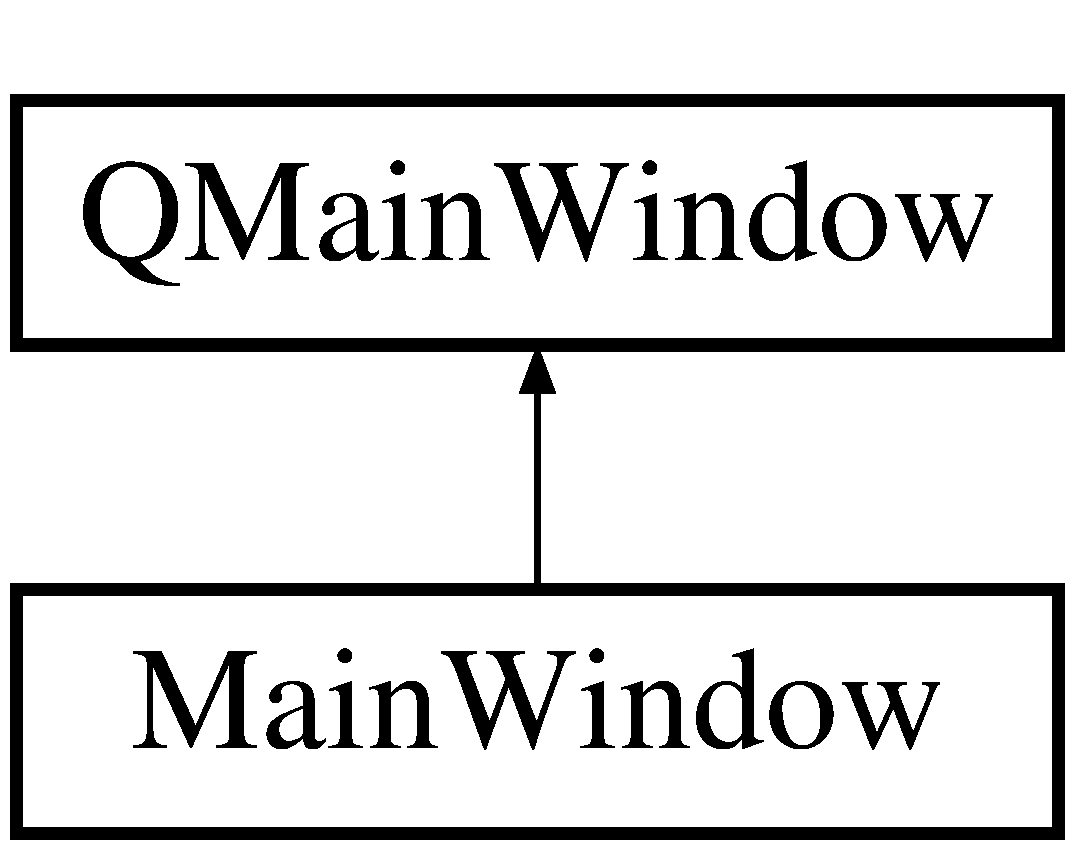
\includegraphics[height=2.000000cm]{class_main_window}
\end{center}
\end{figure}
\subsection*{Public Member Functions}
\begin{DoxyCompactItemize}
\item 
{\bfseries Main\+Window} (Q\+Widget $\ast$parent=0)\hypertarget{class_main_window_a8b244be8b7b7db1b08de2a2acb9409db}{}\label{class_main_window_a8b244be8b7b7db1b08de2a2acb9409db}

\end{DoxyCompactItemize}


The documentation for this class was generated from the following files\+:\begin{DoxyCompactItemize}
\item 
C\+:/\+Users/muell/\+One\+Drive/\+U\+N\+I/2. Semester/\+Informatik 2/\+Projekt/qt\+\_\+\+Projekt/\+Temp\+Monitor/mainwindow.\+h\item 
C\+:/\+Users/muell/\+One\+Drive/\+U\+N\+I/2. Semester/\+Informatik 2/\+Projekt/qt\+\_\+\+Projekt/\+Temp\+Monitor/mainwindow.\+cpp\end{DoxyCompactItemize}

\hypertarget{class_serial}{}\section{Serial Class Reference}
\label{class_serial}\index{Serial@{Serial}}
\subsection*{Public Member Functions}
\begin{DoxyCompactItemize}
\item 
void {\bfseries open} (Q\+String port\+Name)\hypertarget{class_serial_a8bfba783b2b4988c43d1347149ee164f}{}\label{class_serial_a8bfba783b2b4988c43d1347149ee164f}

\item 
void {\bfseries close} ()\hypertarget{class_serial_afbe59407e718bc3d22ea4a67b304db6c}{}\label{class_serial_afbe59407e718bc3d22ea4a67b304db6c}

\end{DoxyCompactItemize}


The documentation for this class was generated from the following files\+:\begin{DoxyCompactItemize}
\item 
C\+:/\+Users/muell/\+One\+Drive/\+U\+N\+I/2. Semester/\+Informatik 2/\+Projekt/qt\+\_\+\+Projekt/\+Temp\+Monitor/serial.\+h\item 
C\+:/\+Users/muell/\+One\+Drive/\+U\+N\+I/2. Semester/\+Informatik 2/\+Projekt/qt\+\_\+\+Projekt/\+Temp\+Monitor/serial.\+cpp\end{DoxyCompactItemize}

\hypertarget{class_temp}{}\section{Temp Class Reference}
\label{class_temp}\index{Temp@{Temp}}


{\ttfamily \#include $<$temp.\+h$>$}

\subsection*{Public Member Functions}
\begin{DoxyCompactItemize}
\item 
{\bfseries Temp} (double t, Q\+Date\+Time time, int i)\hypertarget{class_temp_ac0cb3f11a2a9c9b4175d2867ba50e499}{}\label{class_temp_ac0cb3f11a2a9c9b4175d2867ba50e499}

\end{DoxyCompactItemize}
\subsection*{Public Attributes}
\begin{DoxyCompactItemize}
\item 
double {\bfseries temp}\hypertarget{class_temp_a599fd6c9646291de791fde0b8b2553e6}{}\label{class_temp_a599fd6c9646291de791fde0b8b2553e6}

\item 
Q\+Date\+Time {\bfseries timestamp}\hypertarget{class_temp_af7e6ec5c6aac775b855491ff26531de3}{}\label{class_temp_af7e6ec5c6aac775b855491ff26531de3}

\item 
int {\bfseries interval}\hypertarget{class_temp_a01725bdf952fc8aeb9e3ec4238ef4e8c}{}\label{class_temp_a01725bdf952fc8aeb9e3ec4238ef4e8c}

\end{DoxyCompactItemize}


\subsection{Detailed Description}
A class for storing a dataset of a temperature value and a timestamp 

The documentation for this class was generated from the following files\+:\begin{DoxyCompactItemize}
\item 
C\+:/\+Users/muell/\+One\+Drive/\+U\+N\+I/2. Semester/\+Informatik 2/\+Projekt/qt\+\_\+\+Projekt/\+Temp\+Monitor/temp.\+h\item 
C\+:/\+Users/muell/\+One\+Drive/\+U\+N\+I/2. Semester/\+Informatik 2/\+Projekt/qt\+\_\+\+Projekt/\+Temp\+Monitor/temp.\+cpp\end{DoxyCompactItemize}

%--- End generated contents ---

% Index
\backmatter
\newpage
\phantomsection
\clearemptydoublepage
\addcontentsline{toc}{chapter}{Index}
\printindex

\end{document}
